%% TRCS - Tokenized Reward & Credential System
%% Project Proposal Document
%% 1-2 Pages

\documentclass[12pt,a4paper]{article}

%% Packages
\usepackage[utf8]{inputenc}
\usepackage[T1]{fontenc}
\usepackage{lmodern}
\usepackage[margin=1in]{geometry}
\usepackage{graphicx}
\usepackage{xcolor}
\usepackage{hyperref}
\usepackage{enumitem}
\usepackage{tikz}
\usepackage{booktabs}

%% TikZ Libraries
\usetikzlibrary{shapes.geometric, arrows, positioning, fit}

%% Colors
\definecolor{primaryblue}{RGB}{41, 98, 255}
\definecolor{secondarygreen}{RGB}{0, 200, 83}

\hypersetup{
    colorlinks=true,
    linkcolor=primaryblue,
    urlcolor=primaryblue,
    pdftitle={TRCS Project Proposal},
    pdfauthor={Samir Guenchi},
}

%% Title
\title{
    \vspace{-1cm}
    \textbf{Project Proposal}\\[0.3cm]
    \Large Tokenized Reward \& Credential System (TRCS)\\[0.2cm]
    \large Reward and Certify Student Participation in\\
    Workshops, Competitions, and Club Events
}
\author{Samir Guenchi}
\date{December 2025}

\begin{document}

\maketitle

%% ============================================
\section{Purpose}
%% ============================================

The \textbf{Tokenized Reward \& Credential System (TRCS)} is a blockchain-based platform designed to reward and certify student participation in campus activities such as:

\begin{itemize}[nosep]
    \item \textbf{Workshops} -- Technical training sessions, skill-building seminars
    \item \textbf{Competitions} -- Hackathons, coding contests, innovation challenges
    \item \textbf{Club Events} -- Student organization meetings, community service, conferences
\end{itemize}

\subsection{Problem Statement}
Traditional participation tracking systems suffer from:
\begin{enumerate}[nosep]
    \item \textbf{Lack of verifiability} -- Paper certificates can be forged or lost
    \item \textbf{No tangible incentives} -- Students lack motivation to participate
    \item \textbf{Centralized control} -- Records depend on institutions that may lose data
    \item \textbf{No portability} -- Achievements don't transfer between institutions
\end{enumerate}

\subsection{Solution}
TRCS solves these problems by:
\begin{itemize}[nosep]
    \item Issuing \textbf{ERC-721 NFT credentials} as tamper-proof participation certificates
    \item Distributing \textbf{ERC-20 TRCS tokens} as rewards for completing activities
    \item Storing all records on-chain for \textbf{permanent, decentralized verification}
    \item Enabling students to \textbf{own and control} their achievements via crypto wallets
\end{itemize}

%% ============================================
\section{System Architecture}
%% ============================================

\begin{center}
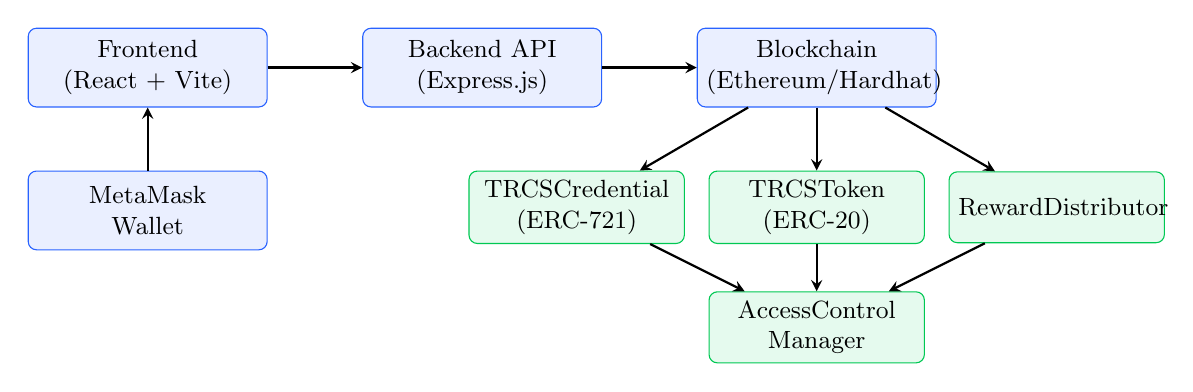
\begin{tikzpicture}[
    node distance=1.2cm,
    box/.style={rectangle, draw=primaryblue, fill=primaryblue!10, text width=2.8cm, align=center, minimum height=1cm, rounded corners=3pt, font=\small},
    contract/.style={rectangle, draw=secondarygreen, fill=secondarygreen!10, text width=2.5cm, align=center, minimum height=0.9cm, rounded corners=3pt, font=\small},
    arrow/.style={->, thick, >=stealth}
]

% Frontend
\node[box] (frontend) {Frontend\\(React + Vite)};

% Backend
\node[box, right=of frontend] (backend) {Backend API\\(Express.js)};

% Blockchain
\node[box, right=of backend] (blockchain) {Blockchain\\(Ethereum/Hardhat)};

% Smart Contracts
\node[contract, below=0.8cm of blockchain] (token) {TRCSToken\\(ERC-20)};
\node[contract, left=0.3cm of token] (credential) {TRCSCredential\\(ERC-721)};
\node[contract, right=0.3cm of token] (reward) {RewardDistributor};
\node[contract, below=0.6cm of token] (access) {AccessControl\\Manager};

% Wallet
\node[box, below=0.8cm of frontend] (wallet) {MetaMask\\Wallet};

% Arrows
\draw[arrow] (frontend) -- (backend);
\draw[arrow] (backend) -- (blockchain);
\draw[arrow] (wallet) -- (frontend);
\draw[arrow] (blockchain) -- (token);
\draw[arrow] (blockchain) -- (credential);
\draw[arrow] (blockchain) -- (reward);
\draw[arrow] (token) -- (access);
\draw[arrow] (credential) -- (access);
\draw[arrow] (reward) -- (access);

\end{tikzpicture}
\end{center}

\subsection{Technology Stack}

\begin{table}[h]
\centering
\begin{tabular}{@{}lll@{}}
\toprule
\textbf{Layer} & \textbf{Technology} & \textbf{Purpose} \\
\midrule
Blockchain & Solidity 0.8.20 & Smart contract language \\
Development & Hardhat & Testing \& deployment \\
Backend & Express.js + ethers.js & API \& blockchain interaction \\
Frontend & React + TypeScript & User interface \\
Wallet & MetaMask & User authentication \\
\bottomrule
\end{tabular}
\end{table}

%% ============================================
\section{Smart Contracts}
%% ============================================

The system consists of four interconnected smart contracts:

\subsection{AccessControlManager.sol}
Manages role-based permissions using OpenZeppelin's AccessControl pattern.
\begin{itemize}[nosep]
    \item \texttt{ADMIN\_ROLE} -- Full system control
    \item \texttt{ISSUER\_ROLE} -- Can issue credentials
    \item \texttt{DISTRIBUTOR\_ROLE} -- Can distribute token rewards
\end{itemize}

\subsection{TRCSToken.sol (ERC-20)}
The reward token with the following features:
\begin{itemize}[nosep]
    \item \textbf{Symbol:} TRCS | \textbf{Decimals:} 18 | \textbf{Cap:} 100,000,000
    \item Mintable by authorized distributors
    \item Burnable by token holders
    \item Transfer pause capability for emergencies
\end{itemize}

\subsection{TRCSCredential.sol (ERC-721)}
NFT credentials representing participation certificates:
\begin{itemize}[nosep]
    \item Unique token ID per credential
    \item Metadata URI linking to IPFS/on-chain data
    \item Credential types: Course Completion, Skill Certification, Achievement Badge, Membership
    \item Expiration dates for time-limited credentials
    \item On-chain verification of authenticity
\end{itemize}

\subsection{RewardDistributor.sol}
Manages token distribution with vesting:
\begin{itemize}[nosep]
    \item Create vesting schedules for gradual token release
    \item Cliff periods before tokens become claimable
    \item Linear vesting over configurable duration
    \item Direct reward transfers for immediate distribution
\end{itemize}

%% ============================================
\section{Key Features}
%% ============================================

\begin{enumerate}[nosep]
    \item \textbf{Event Participation Tracking} -- Record attendance at workshops, hackathons, club events
    \item \textbf{Automatic Reward Distribution} -- Tokens sent upon activity completion
    \item \textbf{NFT Credential Minting} -- Verifiable certificates stored on blockchain
    \item \textbf{Vesting Schedules} -- Gradual token release to encourage continued participation
    \item \textbf{Wallet-Based Identity} -- Students authenticate via MetaMask, no passwords needed
    \item \textbf{Decentralized Verification} -- Anyone can verify credentials on-chain
\end{enumerate}

%% ============================================
\section{Repository}
%% ============================================

\begin{center}
\url{https://github.com/Samir-Guenchi/Tokenized-Reward-Credential-System}
\end{center}

\end{document}
